%%%%%%%%%%%%%%%%%%%%%%%%%%%%%%%%%%%%%%%%%%%%%%%%%%%%%%%%%%%%%%%%%%% 
%                                                                 %
%                             Animation                           %
%                                                                 %
%%%%%%%%%%%%%%%%%%%%%%%%%%%%%%%%%%%%%%%%%%%%%%%%%%%%%%%%%%%%%%%%%%% 
 
\chapter{ANIMATION}
\label{chapter:animation}

Jumping is the acceleration of a character's center of mass upward.  This motion can be divided into several stages.  First is the lead-up or wind-up stage in which the character flexes or gathers momentum to perform the jump.  This takes the form of a slight crouch (TODO reference cat jumping paper or the background section.  should this be in background?) which prepares the character to exert the necessary force against the ground.  

Next comes the take-off stage.  The character pushes against the floor with their feet, accelerating their center of mass to break contact with the floor.  

\section{Path Estimation}

\begin{figure}[ht]
	\label{fig:pathEstimate}
	\centering
	\begin{tikzpicture}[node distance=1cm and 1cm, auto]
% Path Estimate Phase
	%	Path Estimate Stage
    \node [stage] (path) {\nodebox{5cm}{Path Estimate \[a = \dfrac{2 (x - x_0 - v_0 t)}{t^2} \]}};
    %	Path Estimate Data
    \node [data, above= of path] (xf) {\nodebox{2cm}{Target Position ($x$)}};
    \node [data, left= of xf] (xi) {\nodebox{2cm}{Initial Position ($x_0$)}};
    \node [data, left= of xi](t) {\nodebox{2cm}{Time ($t$)}};
    \node [data, right= of xf] (vi) {\nodebox{2cm}{Initial Velocity ($v_0$)}};
    \node [data, below= of path] (accel) {\nodebox{3cm}{Target Acceleration ($a$)}};
    
    \path [line] (xi) |- (path);
    \path [line] (xf) -- (path);
    \path [line] (t) |- (path);
    \path [line] (vi) |- (path);
    \path [line] (path) -- (accel);
\end{tikzpicture}
	\caption{Diagram of the path estimation step.}
\end{figure}

\begin{figure}[ht]
	\label{fig:pathExample}
	\caption{Example of a path estimation.}
\end{figure}
Before calculations relating to the model's skeleton are performed, an initial estimate of the jump path is performed.  The estimate uses a simple forward kinematic calculation to determine the force required to move an object through the air from the initial position of the model, denoted as $x_0$ in Figure \ref{fig:pathEstimate}, to a final position, denoted as $x$.  To facilitate a character jumping while moving, the path estimate takes into account the initial velocity $v_0$.

The user specifies a desired time ($t$), which indicates the time the character will spend airborne during the animation, i.e. the time between when the character's feet break contact with the ground and when they regain contact with the ground.  This is useful as the desired animation can be more easily adjusted to fit a desired time as an in-game animation or to fit a particular storyboard for an animated film sequence.

\section{Windup}
From this force, the acceleration can be determined using $F=ma$ from classical mechanics.  This assumes the character is a rigid body with negligible air resistance acted upon by gravity of $10\frac{m}{s}$.  The mass is calculated as the summed total of the distributed masses assigned to the character's limbs, which are summed to produce a total mass for the character.

Proportional derivative control is used to produce the windup motion once the initial path estimate is calculated.  The error function $E_{all}$ calculates error from the desired force $E_{force}$ as well as the balance $E_{balance}$.

Once computed, error is compared to a threshold ($\epsilon$).  If the error is below the threshold, the skeleton is considered bent to the proper position for windup and the system proceeds to the thrust phase in which the character unbends.  If the value is above the threshold, a new position for the hip is calculated using proportional-derivative control, where the new position for the iteration of the controller, $u(i)$, is calculated as \[u(i) = k_p E_{all}(i - 1) + k_d(E_{all}(i-1) - E_{all}(i-2))\] where $i$ is the iteration, and $k_p$ and $k_d$ are weights which determine the rate of change. This new hip position is given to an inverse kinematics component to calculate the positions of the remaining leg joints, assuming the feet should remain in the same position.  These new joint positions and angles are then passed back to the PD controller to re-calculate the center of mass as well as the new force and balance errors for the next iteration.

\begin{figure}[ht]
	\label{fig:bendPhase}
	\centering
	\resizebox{\textwidth}{!}{
		\begin{tikzpicture}[node distance = 0.5cm, auto]
% Bend Phase
    % before controller, need to calculate the desired 
    % place nodes
    \node [data, below of=path] (accel) {\nodebox{2.5cm}{Target Acceleration ($a$)}};
	\node [data, left=of accel] (mass) {\nodebox{3.5cm}{Body Mass assigned to each limb ($\left\lbrace m_0, \ldots, m_n\right\rbrace$)}};
    \node [stage, below= of accel] (forceCalc) {\nodebox{6cm}{Calculate desired force $F_{target} = \displaystyle\sum_{j=0}^n {m_j} a$}};
    % connecting lines
    \path [line] (accel) -- (forceCalc);
    \path [line] (mass) |- (forceCalc);
    % ----------------
	
    % PD controller
    % place nodes
    \node [substage, below=5cm of forceCalc] (bendErr) {Calculate error from desired force magnitude ($E_{force}$)};
    \node [substage, left=2.5cm of bendErr] (bendBal) {Calculate balance error ($E_{balance}$)};
    \node [substage, above=1cm of bendBal] (comCalc) {\nodebox{5cm}{Calculate Center of Mass \[C_{mass} = \displaystyle\sum_{\forall m} m \cdot position(m)\]}};
    \node [data, below left=1cm and -2cm of bendErr] (bendErrAll) {\nodebox{4cm}{$E_{all} = E_{force} + E_{balance}$}};
    \node [decision, below=0.5cm of bendErrAll] (bendPDTest) {$E_{all} \overset{?}{\le} \epsilon$};
    \node [substage, left=1cm of bendPDTest] (bendPDEq) {Set new hip position based on $u(i) = k_p E_{all}(i-1) + k_d \left(E_{all}(i-1) - E_{all}(i-2)\right)$};
    \node [stage, label={[shift={(-0.5cm, 2cm)}, rotate=90]180:\LARGE PD Controller}, fit=(comCalc) (bendErr) (bendBal) (bendErrAll) (bendPDEq) (bendPDTest)] (bendPD) {};
    \node [data, below=2cm of bendPDTest] (bentSkel) {\nodebox{3cm}{Skeleton in bent position ($\theta_{x} \forall x \in J_m$)}};
    \node [data, below=1cm of bendPDEq] (bendPDConst) {
    \nodebox{4cm}{Proportional and Derivative weights ($k_p, k_d$)}};
    % connecting lines
	\path [line] (forceCalc) -- (bendErr);
	\path [line] (comCalc) -- (bendBal);
	\path [line] (bendErr) |- (bendErrAll);
    \path [line] (bendBal) |- (bendErrAll);
    \path [line] (bendErrAll) -- (bendPDTest);
    \path [line] (bendPDTest) -- (bendPDEq);
    \path [line] (bendPDTest) -- (bentSkel);
    \path [line] (bendPDConst) -- (bendPDEq);
    % ----------------
    
    % CoM inputs
    % place nodes
    \node [data, above =2cm of comCalc] (skeleton) {\nodebox{2.5cm}{Model with skeleton attached ($J = \left\lbrace j_0, \ldots, j_n \right\rbrace$, contains at least a pelvis and both left and right hips, knees, ankles, heels, and toes)}}; 
    \node [data, left=1cm of skeleton] (mjoints){\nodebox{3cm}{Muscled joints ($J_m = \lbrace$ $j_{pelvis}$, $j_{Lhip}$, $j_{Rhip}$, $j_{Lknee}$, $j_{Rknee}$, $j_{Lankle}$, $j_{Rankle}$, $j_{Lheel}$, $j_{Rheel}$, $j_{Ltoe}$, $j_{Rtoe}$ $\rbrace$}};
    \node [data, left=1cm of mjoints] (muscles) {\nodebox{3cm}{Muscle spring constant for muscled joints ($\left\lbrace k_0, \ldots, k_11\right\rbrace$)}};
	\node [data, left=1cm of muscles] (jconst) {\nodebox{2cm}{Rotation constraints for joints ($\theta_{min}, \theta_{max}$ $\forall j \in J_{muscled}$)}};
	
	% connecting lines
	\path [line] (skeleton) -- (comCalc);
	\path [line] (mjoints) -- ++(0cm, -3.4cm) -| (comCalc);
	\path [line] (muscles) -- ++(0cm, -3.5cm) -| (comCalc);
	\path [line] (jconst) -- ++(0cm, -3.6cm) -| (comCalc);
	% ----------------	
	
	% IK solver side stage
	% place nodes
	\node [data, left=3cmof bendPDEq] (IKCurJoint) {\nodebox{4cm}{$R = position(j)$ $\forall j \in J_{ik} \subseteq J$ starting with the root (hip joint).}};
	\node [data, left=1cm of IKCurJoint] (IKTargetPos) {\nodebox{4cm}{Target position for joint, in this case keeping $E$ in it's original position ($D$).}};
	\node [data, left=1cm of IKTargetPos] (IKEndJoint) {\nodebox{2cm}{Joint to move to target ($E$).}};
	\node [data, above=1cm of IKEndJoint] (IKRE) {\nodebox{3cm}{Normalized vector $\vec{RE}$}};
	\node [data] (IKRD) at (IKCurJoint |- IKRE) {\nodebox{3cm}{Normalized vector $\vec{RD}$}};
`	\node [substage, above=2cm of IKTargetPos] (IKEq) {$\theta_j = \vec{RD} \times \vec{RE}$.};
	\node [data, above left=1cm of IKEq] (IKItrs) {\nodebox{3cm}{Number of iterations for IK solver ($num_itr$)}};
	\node [data] (IKPartBent) at (IKEq |- comCalc) {\nodebox{2cm}{Bent skeleton reflecting $u(i)$.}};
	\node [stage, label={[shift={(-0.5cm, 1.5cm)}, rotate=90]180:\LARGE IK Solver}, fit=(IKCurJoint) (IKEndJoint) (IKTargetPos) (IKItrs) (IKRD) (IKEq) (IKPartBent)] (bendIK) {Requires joints to be in a single chain.};
    % connecting lines
    \path [line] (bendPDEq) -- (IKCurJoint);
    \path [line] (IKPartBent) -| ++(6cm, -1.6cm) -| (bendErr);
    \path [line] (IKPartBent) -- (comCalc);
    \path [line] (IKCurJoint) -- (IKRD);
    \path [line] (IKEndJoint) -- (IKRE);
    \path [line] (IKTargetPos) |- (IKRD);
    \path [line] (IKTargetPos) |- (IKRE);
    \path [line] (IKRD) |- (IKEq);
    \path [line] (IKRE) |- (IKEq);
    \path [line] (IKEq) -- (IKPartBent);
    \path [line] (IKItrs) |- (IKEq);
    % ----------------
\end{tikzpicture}
	}
	\caption{Algorithm diagram of the windup phase.}
	%TODO decision lines need to be labeled
\end{figure}

\subsection{Force calculation}
% calculation of the muscle flexion
\begin{figure}[ht]
	\label{fig:forceCalc}
	\centering
	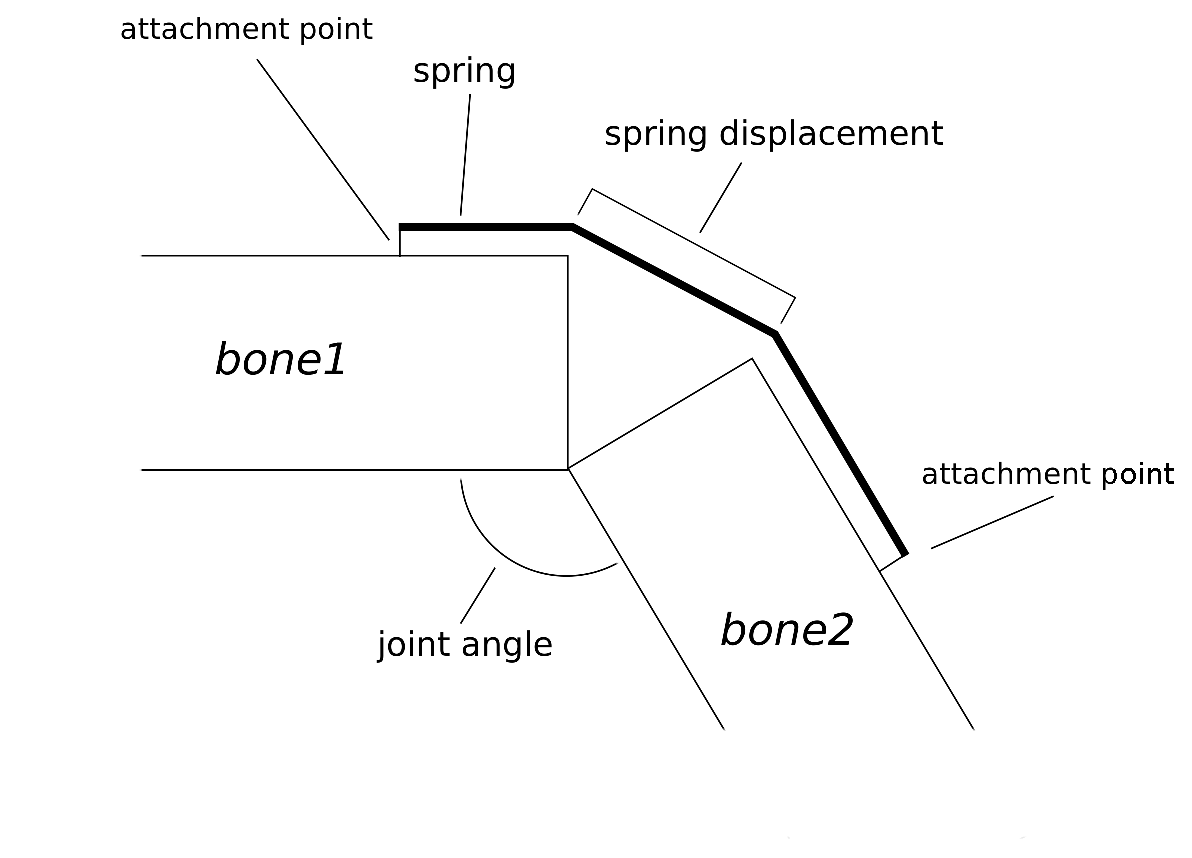
\includegraphics[width=10cm]{images/spring_calc/spring_angle_calc.eps}
	\caption{Force calculation for a joint.}
\end{figure}
Current force is computed by approximating muscles as linear springs attached to two bones and crossing a joint.  The change in spring length is produced by the bend of the joint which opens a space between the rigid bones that the spring must stretch across.  This approximation uses spring constants that simulate a flexed muscle that has been stretched by an amount equal to \[\theta = cos^{-1} \left( \dfrac{2 k^2 r^2}{F^2} - 1 \right)\] which requires a more rigid spring constant.  In this equation, $r$, represents the width of the bone, which is a constant that changes the amount the character must bend to achieve a force.  This acts similarly to the $k$ value, which represents the stiffness of the spring, or a constant for the linear restoring force of the muscle.  
%TODO For our simulations, we used values in the range ().
%TODO values and equation
%TODO tables of values with varied k and varied r and corresponding bend/angle
\begin{table}[ht]
	\label{tab:variedSpringValues}
	\centering
	\caption{A table of various values for k and r, demonstrating effect on the model's bend.  TODO Columns of k and r (varied individually), and image of fully bent character resulting from values.}
\end{table}

At each iteration of the PD controller, current force output of the legs is computed in the same way, with the total actual force, $F_{leg}$ computed as \[F_{leg} = F_{ankle} + F_{knee} + F_{hip}\] for each leg, with 
%TODO does this setup effectively result in springs connected in series? No because you can assume that the muscles you don't want to unbend with remain rigid?
%TODO does this give a sort of impulse function as you unbend at the hips and knees, then the ankles?
%TODO this is where the torques come into play, and they're absolutely necessary

\begin{figure}[ht]
	\label{fig:forceErr}
	\centering
	\caption{Force error calculation}
\end{figure}

\subsection{Center of Mass and Balance}
%TODO need to standardize usage of joint to anatomical, animation, or something else
The center of mass is calculated as the centroid of the character.  More specifically, joint positions are averaged, with a weight assigned to each joint based on the weight of the limb associated.  
\begin{figure}[ht]
	\label{fig:balanceErr}
	\centering
	\caption{Balance error calculation.}
\end{figure}



\subsection{Inverse Kinematic Solving}
As the skeleton is a hierarchy assumed to be rooted at the hip, a problem arises with applying rotations to joints.  To keep a character's feet rooted to the floor as is expected, positions must be solved for using inverse kinematics.  Given the desired position for the hip, and the desired position of the foot, the joint angles and positions of the knee and ankle are solved for.  Constraints are placed on each joint, limiting the range of motion to an expected range as well as limiting the axes about which each joint can rotate, preventing unnatural directions of motion.  These values are specified per joint and can be edited by the user to simulate varied levels of flexibility or alternate body shapes.

%TODO alternate body with digitigrade, Tauren or whatever from WoW, raptor style...
%TODO Further justification of why choosing this method instead of learning is that this is more user-tunable as opposed to a learning heavy model which doesn't allow as much user tuning

\begin{table}[ht]
	\label{tab:jointConstraints}
	\centering
	\caption{Joint angle constraint values used for each joint, with accompanying images of expected motion range.}
\end{figure}


\section{Thrust and Takeoff}

\section{Summary}
\label{section:animation_summary}